\chapter{Tecniche di trasmissione}
\label{cha:intro}
\section{Storia dello sviluppo}
\label{sec:context}
 La comunicazione fra gli esseri umani è una delle abilità che hanno permesso all' uomo di evolversi. La prima forma di comunicazione è stata quella verbale, molto rapida ed efficace che però non garantisce la durata delle informazioni trasmesse. Altri metodi di comunicazione vennero sviluppati, alcuni fra i più interessanti erano le nuvole di fumo che venivano utilizzate dagli indigeni d'America e dai cinesi per comunicare lungo la grande muraglia cinese. Analogamente le tribù africane utilizzavano i tamburi. La scrittura apparse circa 7000 anni fa favorendo l'inizio di un progresso che porterà l'uomo verso il ruolo centrale che ha ora sulla terra. Già nell'epoca della nascita di Cristo l'uomo aveva instaurato una rete di comunicazione in forma scritta che interessava tutto il vecchio continente e lo collegava anche al mondo indiano ed orientale. Altri metodi un po' particolari vennero sfruttati prima dell' invenzione dell' elettricità come ad esempio: l'addestramento di piccioni viaggiatori  che dimostrano avere un packet loss di solo il 17\% oppure l'utilizzo di una lingua formata da fischi fra le lunghe valli nelle isole dell'arcipelago delle Canarie.
Con la scoperta della corrente elettrica si è aperto per noi un nuovo mondo di possibilità fra le quali quella di trasferire immense quantità di informazioni velocemente e su lunghe distanze. Dapprima il telegrafo e poi il telefono fino ad arrivare alle trasmissioni analogiche seguite dall'avvento dell'era digitale. Nelle telecomunicazioni moderne per trasmettere si utilizza una portante (segnale elettrico oppure onda elettromagnetica) alla quale vengono aggiunte le informazioni secondo diverse tecniche dette anche modulazioni.


\section{Modulazioni Analogiche}
Le modulazioni analogiche sono utilizzate per inviare un segnale la cui variazione avviene all'interno di un intervallo teoricamente con infiniti impossibili valori. Sono solitamente meno complesse da implementare per il ricevitore rispetto alle versioni digitali.
\label{sec:context}
\begin{itemize}
   	\item \subsection{AM (Amplitude Modulation): } La modulazione in ampiezza è stata una delle prime modulazioni utilizzate grazie alla sua facilità di implementazione in hardware. Il segnale viene direttamente sommato alla portante in modo analogico, la sua semplicità è ormai l'unico vantaggio in quanto una soluzione di questo tipo è soggetta ad interferenze di qualsiasi origine, è sufficiente infatti una semplice attenuazione del segnale per influire direttamente sui dati ricevuti. Questa modulazione viene ancora utilizzata per la trasmissione radio che grazie a frequenze molto basse (khz) e potenze elevate (kw) permette di comunicare su distanze mondiali
   \item \subsection{FM (Frequency Modulation): } La modulazione viene effettuata variando la frequenza del segnale portante alzandola o abbassandola in relazione alle informazioni da trasmettere, è più efficiente della modulazione in ampiezza in quanto non necessita di variare la potenza. Richiede però dei circuiti più complessi che siano in grado di svolgere il compito di codifica/decodifica. La modulazione in frequenza FM è tuttora utilizzata per la trasmissione della radio anche se sta venendo progressivamente sostituita dalla radio digitale "DAB"
   \item \subsection{PM (Phase Modulation): } Le informazioni vengono modulate modificando la fase della portante in relazione al valore di ampiezza del segnale analogico in ingresso. Viene raramente utilizzata a causa della complessità richiesta nei ricevitori, tuttavia il principio di funzionamento alla base è lo stesso utilizzato da PSK e QAM.
  \end{itemize}
  %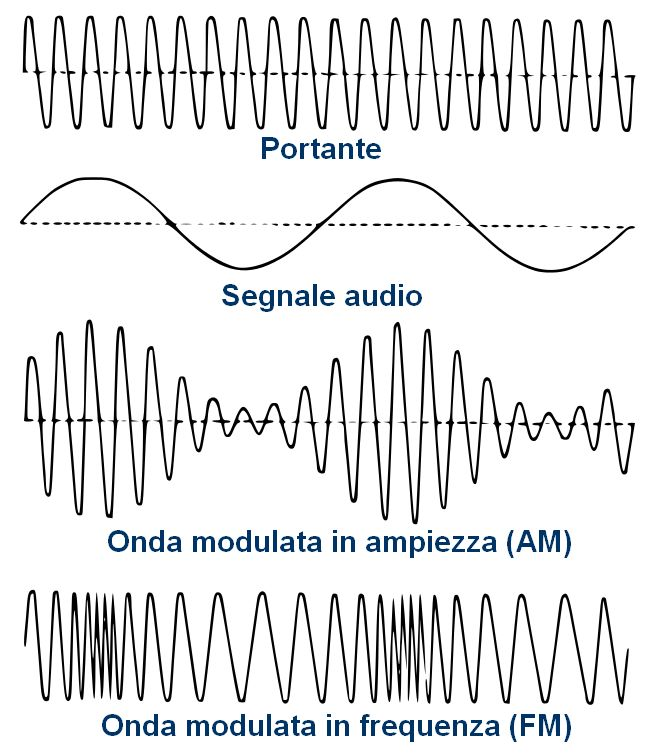
\includegraphics[scale=0.3]{amfm}
\begin{figure}[h]
	\centering
	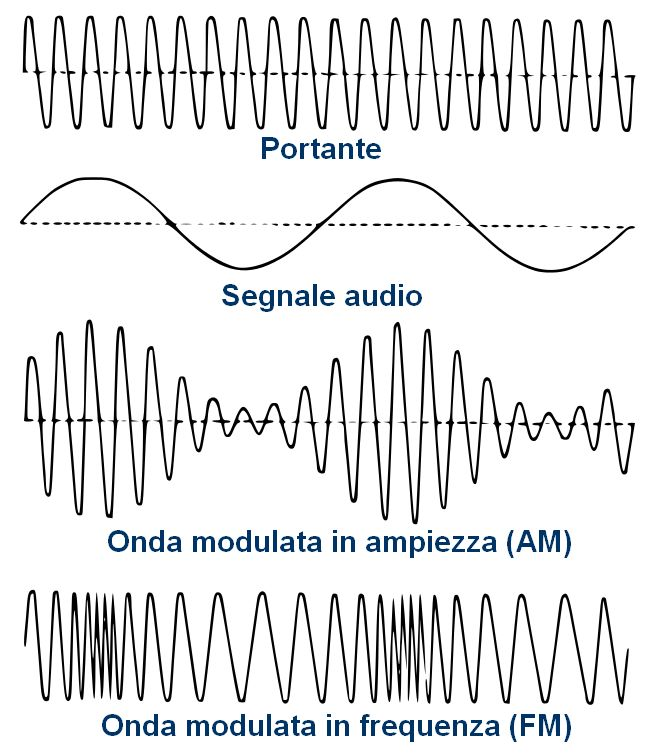
\includegraphics[scale=0.23]{amfm}
	\caption{rappresentazione segnale modulato AM e FM nel tempo}\label{fig:1}
\end{figure}



\section{Modulazioni Digitali}
\label{sec:context}
\begin{itemize}
  \item \subsection{FSK (Frequency Shifting Key): } Questa tecnica di modulazione codifica l'informazione variando la frequenza della portante in valori predefiniti, ad esempio per ottenere una codifica binaria alterna due frequenze diverse. Questa tecnica ha il vantaggio di essere facile nell'implementazione e poco soggetta ad interferenze, tuttavia necessita di una maggiore larghezza di banda rispetto ad altre modulazioni digitali quali psk o ask.
  \cite{fsk}
  \item \subsection{ASK (Amplitude Shift Keying): } La modulazione viene effettuata variando l'ampiezza del segnale portante alzandola o abbassandola in relazione alle informazioni da trasmettere, richiede un canale più affidabile in grado di ricevere anche i livelli di ampiezza più bassi. Trova ancora utilizzo nelle fibre ottiche e la sua versione a codifica binaria (solo due livelli di potenza della portante presente/non presente) che prende il nome di OOF(on/off keying) veniva in passato utilizzata per trasmettere messaggi in codice morse.
  \cite{ask}
  
  \item \subsection{PSK (Phase Shift Keying): } Questo tipo di modulazione codifica le informazioni in ingresso variando la fase della portante, ne esistono varie versioni che differiscono per il numero di valori diversi. La versione più semplice è la binaryPSK che varia di metà periodo mentre versioni come la 4PSK di un quarto e così via per la variante 8PSK e 16PSK. Tali possibili sfasature della portante vengono dette costellazione e vengono di norma rappresentate come coordinate complesse su un grafico. Sulle ascisse si trova la portante, mentre sulle ordinate si trova in quadratura ovvero sfasata di 90°. La lunghezza del vettore fra l'origine e uno dei punti della costellazione rappresenta l'ampiezza del segnale modulato mentre l'angolo rappresenta la sfasatura rispetto alla portante. Esiste una variante di 4PSK detta QPSK che differisce per una disposizione della costellazione ruotata di 45°.
  \begin{figure}[h!]
  	\begin{minipage}[b]{.6\columnwidth}
  		\centering
  		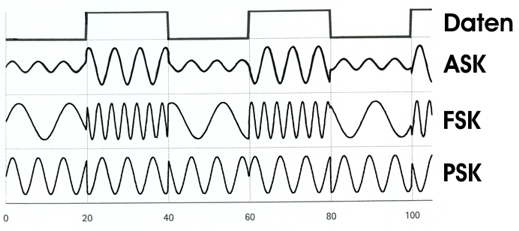
\includegraphics[scale=1.5]{digital}
  		\caption{rappresentazione segnale modulato nel tempo ASK, FSK e PSK \cite{digit}}\label{fig:1}
  	\end{minipage}\hfill
  	\begin{minipage}[b]{.35\columnwidth}
  		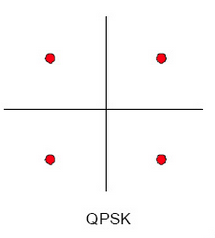
\includegraphics[scale=0.4]{qpsk}
  		\caption{Costellazione QPSK \cite{qpsk}}\label{fig:1}
  	\end{minipage}\hfill
  \end{figure}
  \item \subsection{DPSK (Differential Phase Shift Keying): } Questa tecnica differisce da PSK solo per la particolarità di codificare il simbolo non utilizzando una costellazione fissa, le informazioni sono espresse come cambio di fase rispetto al simbolo precedente. Tale caratteristica rende questa modulazione robusta sia contro variazioni di ampiezza come psk sia contro distorsioni della fase del segnale ricevuto.
  \begin{figure}[h]
  	\centering
  	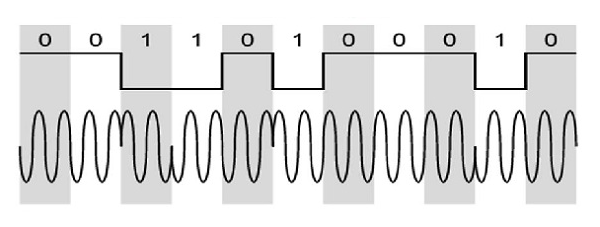
\includegraphics[scale=0.65]{dpsk}
  	\caption{rappresentazione segnale modulato DPSK \cite{dpsk}}\label{fig:1}
  \end{figure}
    
  \item \subsection{QAM (Quadrature Amplitude Modulation): } E' una tecnica di modulazione simile a PSK ma introduce la modulazione anche in ampiezza. La costellazione risulta avere punti non più equidistanti dall'origine. QAM come PSK presenta varianti che differiscono per il numero di punti sulla costellazione, in sistemi moderni si utilizzano anche 256 punti. Una particolarità comune a psk consiste nel fatto che due punti della costellazione adiacente differiscono per un solo bit, ciò incrementa l'efficacia di un eventuale error recovery. QAM viene anche utilizzato per trasferire più flussi analogici contemporaneamente, questo particolare utilizzo fa si che QAM venga considerato anche come una tecnica di modulazione analogica. 
  \cite{qam}
  
  \begin{figure}[h]
	\centering
	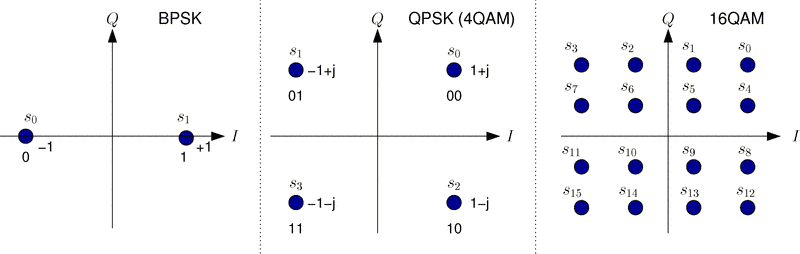
\includegraphics[scale=1.9]{constellation}
	\caption{Costellazioni BPSK, QPSK(4QAM), 16PSK \cite{psk-constellation}}\label{fig:1}
  \end{figure} 
  \end{itemize}
  %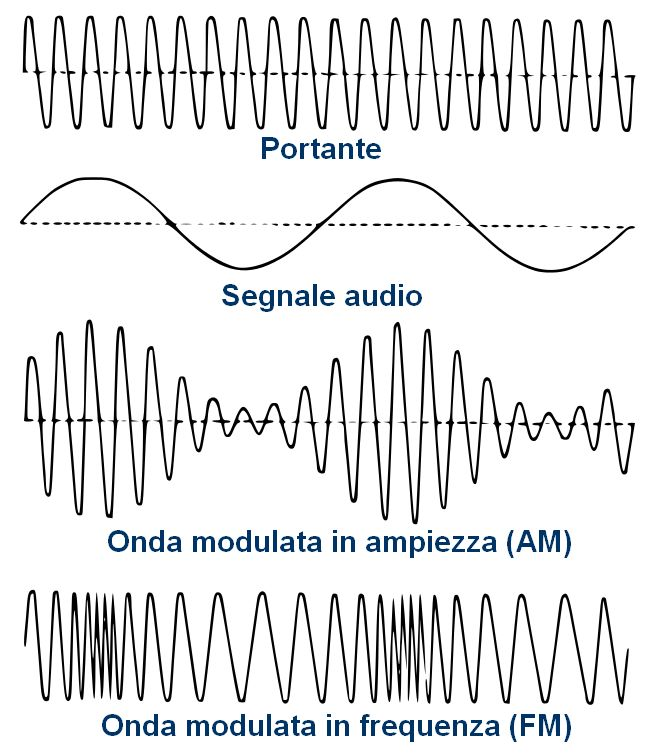
\includegraphics[scale=0.3]{amfm}
\newpage

\chapter{OFDM (Orthogonal Frequency-division Multiplexing): }
OFDM è una tecnica di codifica digitale su portanti multiple, su ogni sotto portante vengono modulate le informazioni utilizzando una delle varie tecniche digitali disponibili (solitamente si utilizza una versione di PSK oppure di QAM). OFDM trova svariati utilizzi nei sistemi di comunicazione moderni come ad esempio adsl, fibra ottica, 4G, wi-fi(802.11a/g/n/ac), radio/televisione digitale e WiMAX.
\cite{ofdm}
\cite{ofdm2}

\label{sec:problem}
\section{Principi di funzionamento}
\begin{itemize}
	 \item \subsection{Ortogonalità delle sottoportanti: } La divisione della larghezza di banda disponibile in sezioni più piccole non è una caratteristica unica di OFDM, ciò che lo distingue è la soluzione al problema di interferenza fra i sotto canali. La soluzione classica è quella di lasciare delle piccole bande di frequenza vuote dove non si trasmette fra un canale e quello adiacente (bande di guardia). Da notare che in questo tipo di approccio si ha una allocazione inefficiente della larghezza di banda disponibile. OFDM utilizza la proprietà di ortogonalità per riuscire a sovrapporre parzialmente canali adiacenti evitando sprechi di banda e aumentando così l'efficienza spettrale ( indica la bontà del sistema nello sfruttare in maniera più o meno efficiente la banda disponibile \cite{efficienzaSpettrale}).
	 La spiegazione matematica di questa tecnica è complessa e fa uso della trasformata di Fourier, è tuttavia possibile intuirne il funzionamento dalla Figura 2.1. L'immagine rappresenta la disposizione delle sotto portanti, sulle ascisse troviamo le frequenze mentre sulle ordinate l'ampiezza. Ogni picco rappresenta un simbolo modulato sulla rispettiva portante. E' possibile notare che in questa particolare disposizione il rumore, che genererebbe ogni sottocanale all'esterno della propria banda, si annulla esattamente in corrispondenza delle frequenze di trasmissione dei simboli adiacenti non causandogli disturbo. Affinché l'ortogonalità garantisca che non ci siano interferenze fra le diverse sottoportanti è necessario che il tempo di trasmissione dei simboli sia uguale in tutto il sistema, in ambienti caratterizzati da una variazione dell'attenuazione sul mezzo trasmissivo (ad esempio sul doppino adsl) un eventuale algoritmo finalizzato ad aumentare il throughput non potrà agire sulla velocità di trasmissione dei simboli ma sul numero di sottoportanti oppure sulla tipologia di costellazione utilizzata per modulare (passando ad esempio da un bpsk che trasferisce un bit per simbolo a 16psk che ne trasferisce 4). Altro requisito fondamentale che verrà approfondito nella sezione dedicata alla sincronizzazione in frequenza è la necessità di avere un ottimo allineamento fra trasmettitore e ricevitore.
	 
	 \begin{figure}[h]
	 	\centering
	 	\begin{minipage}[b]{.50\columnwidth}
	 		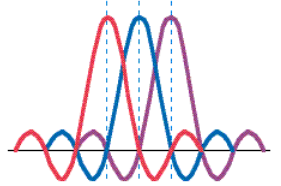
\includegraphics[scale=0.6]{ofdm-simboli}
	 		\caption{Ortogonalità sottoportanti OFDM \cite{ofdm-simboli}}\label{fig:1}
	 	\end{minipage}\hfill
	 	\begin{minipage}[b]{.50\columnwidth}
	 		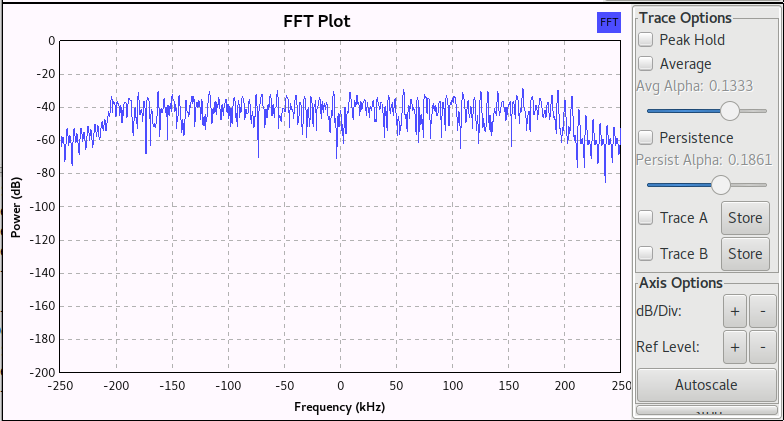
\includegraphics[scale=0.25]{ofdmPie}
	 		\caption{Trasmissione OFDM }\label{fig:1}
	 	\end{minipage}\hfill
	 \end{figure}

 	 \item \subsection{Tempi di guardia } OFDM può soffrire di ISI (inter symbol interference). Questo problema avviene quando un simbolo trasmesso arriva al ricevitore assieme al precedente facendo fallire la decodifica, per risolvere questo problema viene aggiunto un tempo detto di guardia lungo solitamente attorno ad 1/10 del simbolo. Inizialmente durante questo breve intervallo non veniva trasmesso nulla, successivamente è risultato più efficiente trasmette l' ultimo pezzo del simbolo successivo (cyclic prefix) favorendo la corretta decodifica  ricevitore.
 	 \begin{figure}[h]
 	 	\centering
 	 	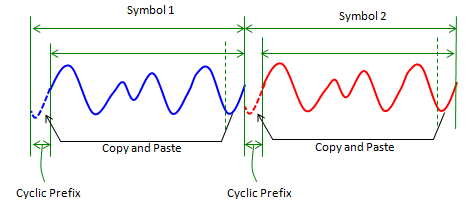
\includegraphics[scale=1]{cp}
 	 	\caption{Cyclic guard \cite{cp}}\label{fig:1}
 	 \end{figure}
     \item \subsection{Equalizzazione} L'equalizzazione del segnale ricevuto è una procedura fondamentale per la corretta decodifica delle informazioni. L'obiettivo di questa procedura è quello di modificare il segnale ricevuto cercando di agire esattamente nel modo opposto di come è stato distorto dal canale in modo da annullarne la distorsione, per ottenere tale risultato esistono numerosi algoritmi di equalizzazione che differiscono per gli approcci diversi in relazione alle informazioni disponibili sul mezzo trasmissivo oppure alle informazioni ottenute durante la trasmissione stessa. Esistono due tipi di equalizzazione possibile uno nel dominio del tempo quindi analizzando lo scorrere dei simboli e uno nel dominio delle frequenze che analizza il comportamento del canale nelle varie sottoportanti. All'inizio di una trasmissione OFDM vengono inviati dei preamboli noti al ricevitore che li utilizza per stimare la distorsione del canale di trasmissione, il ricevitore aggiusta le proprie previsioni anche mentre sta ricevendo grazie ai piloti contenuti in ogni simbolo OFDM. Da notare che l'equalizzatore opera variando in egual modo sia il segnale che il rumore.
     \begin{figure}[h]
     	\centering
     	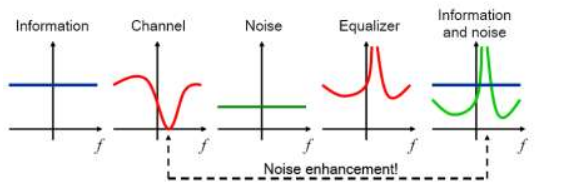
\includegraphics[scale=0.7]{equalizer}
     	\caption{principio funzionamento equalizzatore \cite{equalizer}}\label{fig:1}
     \end{figure}
 \newpage
 \item \subsection{Recupero degli errori} Individuare e correggere gli errori avvenuti nella trasmissione è un compito complesso. Un sistema OFDM necessita la correzione di errore per essere robusto.
 \subsubsection{CRC (Cyclic Redundancy Check)}
 CRC è una tecnica di controllo dell'errore, il funzionamento si basa sull'aggiunta alle informazioni da controllare di un breve codice di controllo. CRC non è in grado di correggere un eventuale errore e non è adatto per verificare la correttezza delle informazioni da un eventuale manomissione. Le informazioni di controllo aggiunte da CRC al messaggio iniziale rappresentano una divisione fra il cosiddetto polinomio generatore (specifico per ogni variante CRC) e il polinomio generato dal messaggio a cui viene sottratto il resto. Anche se di complessa spiegazione questa operazione può essere interamente eseguita in hardware mediante shift register e xor  risultando molto efficiente. Il ricevitore eseguirà la divisione fra il polinomio generatore e il messaggio verificando che il resto sia nullo, se così non fosse il ricevitore è certo che sia presente almeno un errore nelle informazioni ricevute. \cite{crc}
 
 \subsubsection{Convolutional Coding}OFDM può utilizzare CC (Convolutional coding) per la deteminazione e a differenza di CRC la correzione dell'errore. Il principio di funzionamento di questo algoritmo si basa sulla creazione di un diagramma a stati che permette di codificare non solo la sequenza di bit in ingresso ma anche la loro transizione di stato. Il rapporto fra quantità di bit in ingresso e quello in uscita è detto code rate e può variare a seconda delle ciscostanze, un code rate di 1/2 ad esempio aggiunge 1 bit ogni bit in ingresso mentre con un rapporto 4/5 viene aggiunto un bit ogni 4. Meno bit aggiunti si traduce in meno bit da inviare ma minore efficacia nella correzione d'errore \cite{cc}.
 Spesso in OFDM la tecnica di Convolutional coding viene utilizzata assieme ad altre tecniche di recupero errore più complesse come ad esempio Reed-Solomon in grado di recuperare ulteriormente informazioni danneggiate.
 E' bene puntualizzare che esiste un limite, matematicamente dimostrato, insuperabile alla quantità di informazioni trasferibili su un canale affetto da rumore, questo limite è detto di Shannon.
 \cite{ofdmWiki}
 \begin{figure}[h]
 	\centering
 	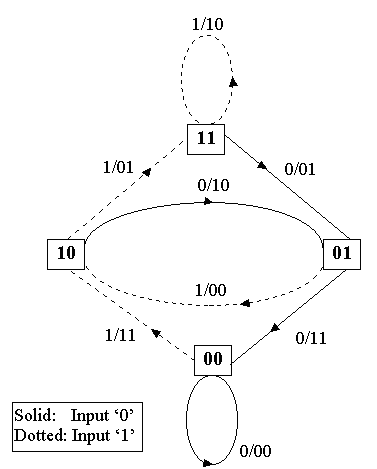
\includegraphics[scale=0.4]{ccDiagram}
 	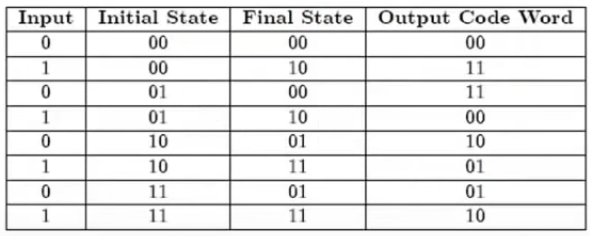
\includegraphics[scale=0.4]{ccTable}
 	\caption{Diagramma a stati e tabella utilizzati per un implementazione di un codificatore CC con output di lunghezza doppia rispetto all'input.}\label{fig:1}
 \end{figure}
\newpage
 \item \subsection{Sincronizzazione in frequenza}
 Lo sfasamento in frequenza fra trasmettitore e ricevitore è un problema comune a tutte le telecomunicazioni. OFDM ne è particolarmente sensibile data la necessità di mantenere l'ortogonalità fra le sottoportanti, altrimenti si manifestano fenomeni non desiderati come l'ICI (Inter Carrier Interference) oppure sfasature del segnale modulato.
 Le cause di una cattiva sincronizzazione possono essere varie, una possibile origine è l'effetto Doppler causato dal movimento di un apparato rispetto all'altro durante la comunicazione. Per le trasmissioni wireless si verifica il cosiddetto multi-path, inoltre possono verificarsi imperfezioni sul clock (generatore di frequenza) fra gli apparati.
 \begin{figure}[h]
 	\centering
 	\begin{minipage}[b]{.55\columnwidth}
 		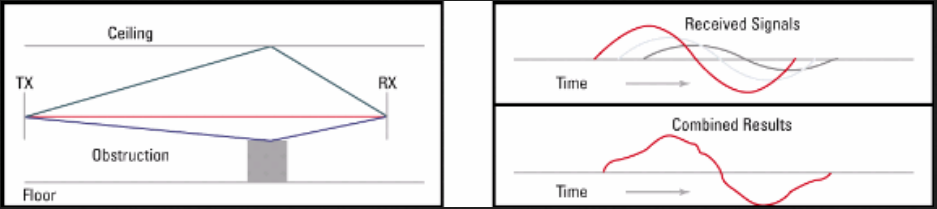
\includegraphics[scale=0.33]{multipath}
 		\caption{Multipath propagation \cite{ofdm-simboli}}\label{fig:1}
 	\end{minipage}\hfill
 	\begin{minipage}[b]{.35\columnwidth}
 		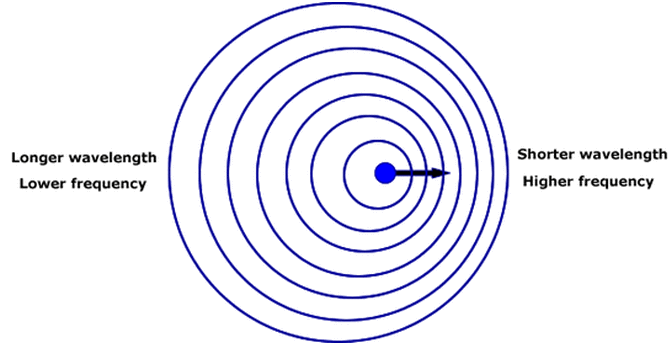
\includegraphics[scale=0.25]{doppler}
 		\caption{Effetto Doppler \cite{doppler}}\label{fig:1}
 	\end{minipage}\hfill
 \end{figure}
 
 
 \subsubsection{Tipologie di sottoportanti}
 Le sottoportanti in OFDM sono classificabili in tre tipologie. La maggior parte sono adibite al trasporto delle informazioni, le restanti sono utilizzate per l'invio di simboli pilota. Esiste un ultima sottoportante particolare che non trasmette nulla (nemmeno la frequenza portante) situata a metà fra tutte le altre che serve al ricevitore per sapere l'esatto centro dell' intera banda.
 \begin{figure}[h]
 	\centering
 	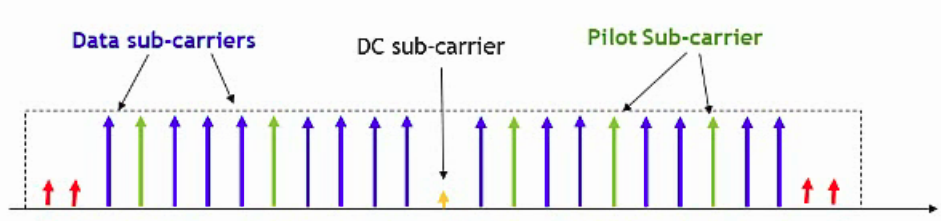
\includegraphics[scale=0.25]{subcarriers}
 	\caption{Tipologie sottopottanti OFDM \cite{subcarriers}}\label{fig:1}
 \end{figure}
  \subsubsection{Trasmissione Preambolo}
	L'invio di dati in OFDM è preceduto da informazioni che vengono utilizzate per la sincronizzazione dal ricevitore. Queste informazioni includono un preambolo e in alcune applicazioni un simbolo contenente alcuni parametri come il numero di simboli OFDM in arrivo.
	\begin{figure}[h!]
		\centering
		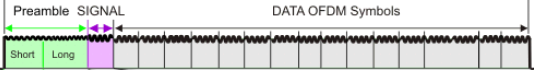
\includegraphics[scale=0.55]{preambolo}
		\caption{Sequenza invio OFDM \cite{subcarriers}}\label{fig:1}
	\end{figure}
 
  Le sfasature in frequenza si dividono principalmente in due tipi, la prima è detta CFO (Carrier Frequency Offset) e rappresenta la sfasatura rispetto alle sottoportanti tra trasmettitore e ricevitore mentre la seconda è nota come SFO (Sampling Frequency Offset) e indica l'errore nella frequenza di campionamento. Il problema del CFO si manifesta in una sfasatura dei campioni ricevuti e viene corretto sincronizzando il ricevitore utilizzando il preabolo (la sua lunghezza determina la precisione). L'SFO si manifesta in una sfasatura dei punti sulla costellazione ed è corretto utilizzando i simboli pilota sempre presenti in alcune specifiche sottoportanti. \cite{FOOFDM}
 %\begin{figure}[h]
 %	\centering
 %	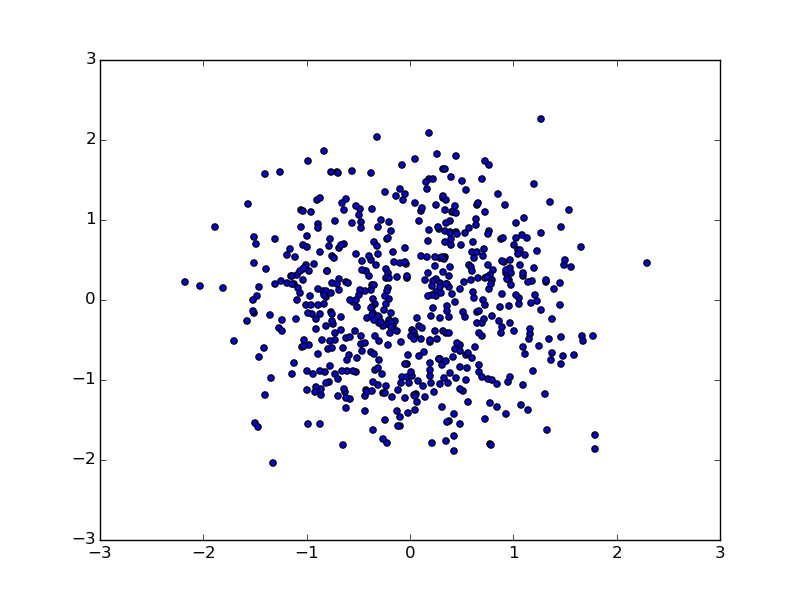
\includegraphics[scale=0.4]{FO0}
 %	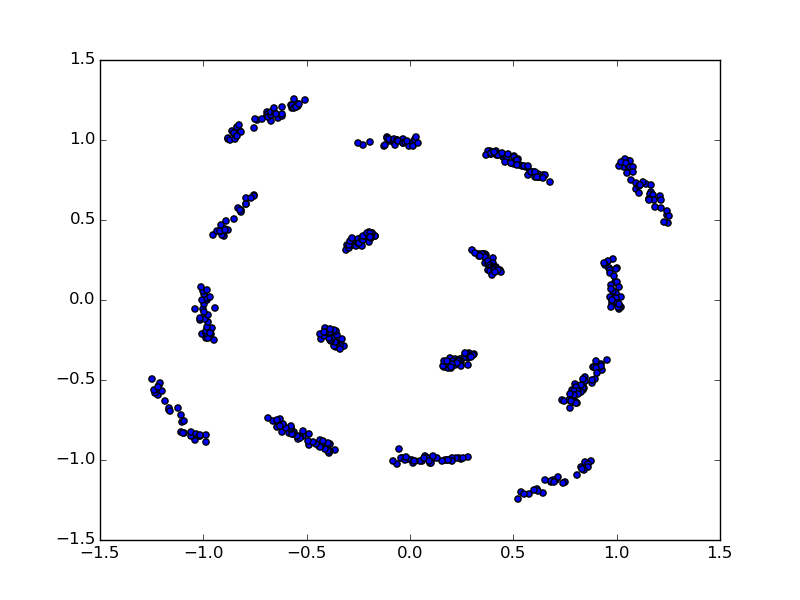
\includegraphics[scale=0.4]{FO1}
 %	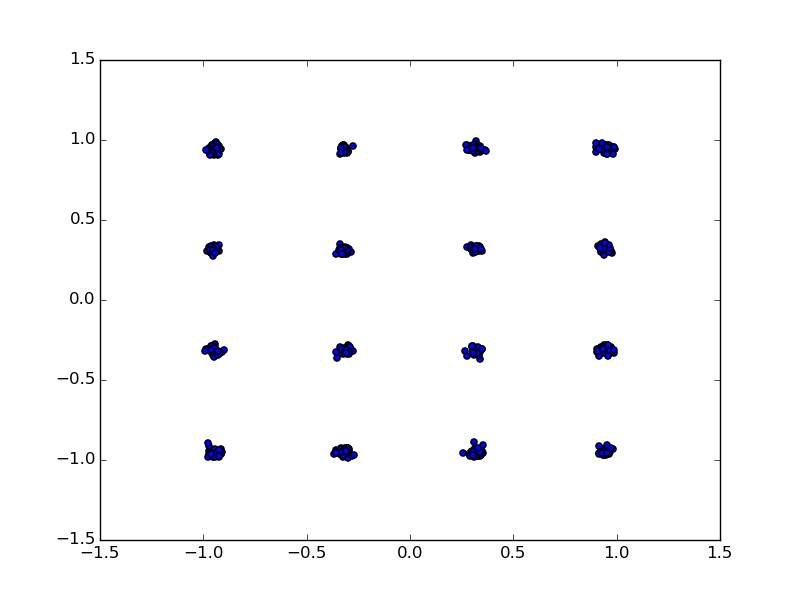
\includegraphics[scale=0.4]{FO2}
 %	\caption{dati grezzi, corretti da CFO con un preambolo corto, corretti da CFO e SFO}\label{fig:1}
 %\end{figure}

\begin{figure}[h]
	\centering
	\begin{minipage}[b]{.30\columnwidth}
		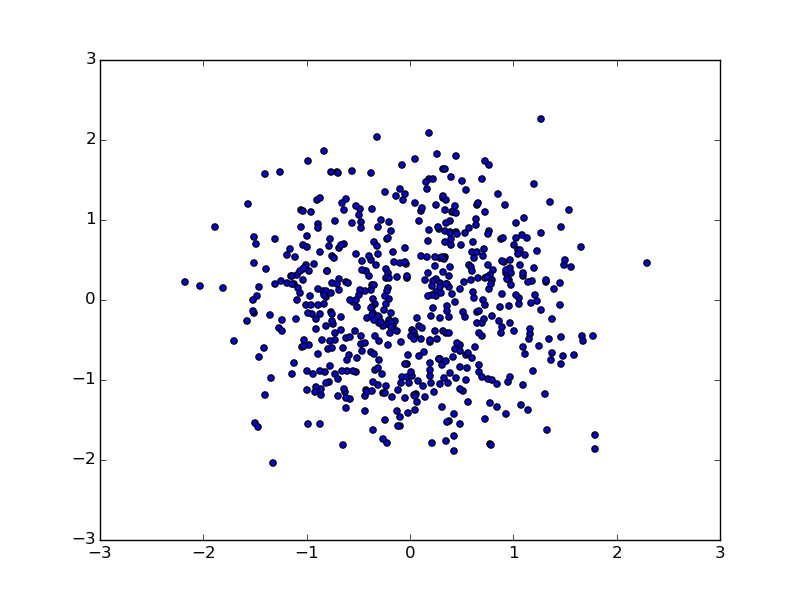
\includegraphics[scale=0.29]{FO0}
		\caption{Costellazione con dati grezzi ricevuti 16QAM}\label{fig:1}
	\end{minipage}\hfill
	\begin{minipage}[b]{.30\columnwidth}
		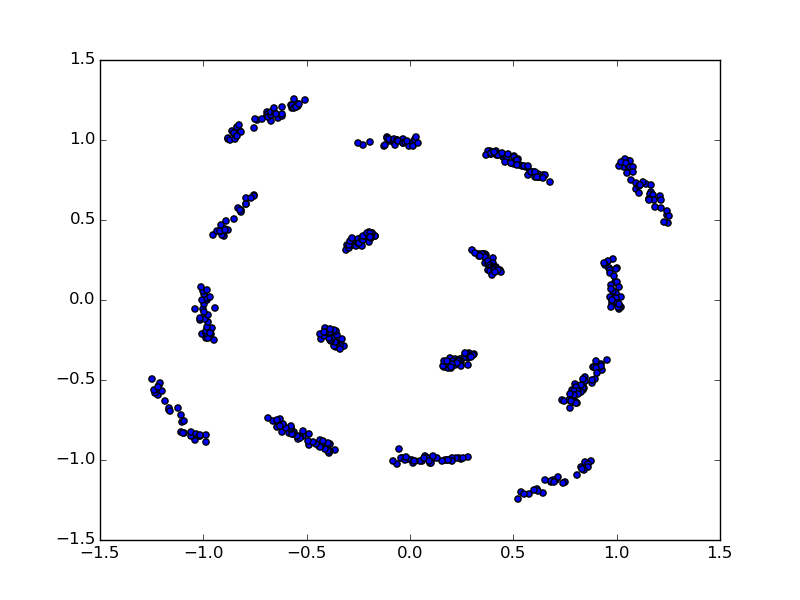
\includegraphics[scale=0.29]{FO1}
		\caption{Corretta da CFO con preambolo corto}\label{fig:1}
	\end{minipage}\hfill
	\begin{minipage}[b]{.30\columnwidth}
		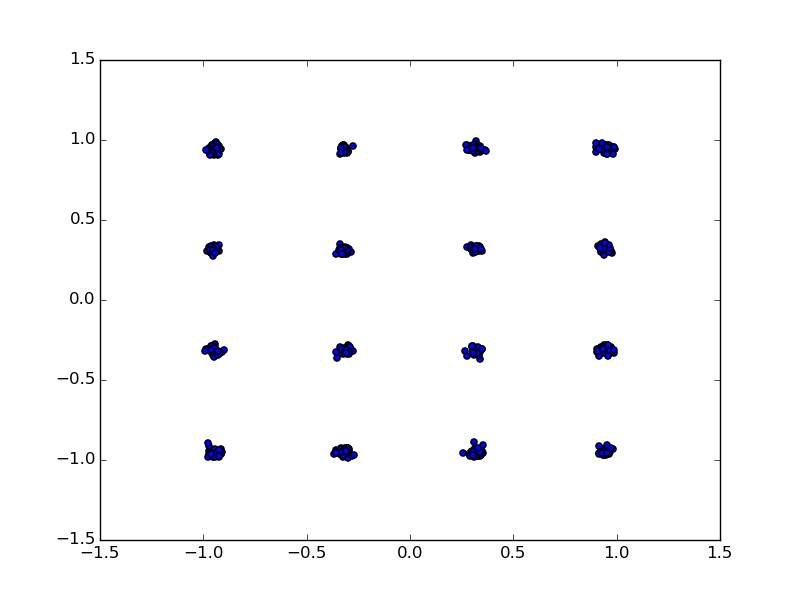
\includegraphics[scale=0.29]{FO2}
		\caption{Corretta da CFO e SFO}\label{fig:1}
	\end{minipage}\hfill
	\cite{FOOFDM}
	\end{figure}
	
	
\label{sec:problem}
\section{Proprietà e campi di utilizzo}
OFDM grazie all'ortogonalità delle portanti permette di avere un ottima efficienza sull'utilizzo della banda, inoltre la scelta (statica o dinamica) del tipo di modulazione da utilizzare in ogni sottoportante lo rende adatto sia in situazioni dove è presente un canale molto distorcente che in casi in cui è desiderabile un elevato throughput. Grazie ai tempi di guardia fra i simboli trasmessi e al prefisso ciclico (Cyclic prefix), OFDM risulta robusto contro il problema della sovrapposizione sul segnale in ricezione di componenti provenienti da segnali riflessi (multipath propagation). OFDM richiede un ottima sincronizzazione e risulta quindi sensibile all'effetto Doppler. OFDM soffre inoltre di un elevato PAPR (peak to average power ratio) causato dalla caratteristica di avere le sottoportanti in quadratura. L'ortogonalità garantisce di non avere sovrapposizioni sulla frequenza dove si trasmette un simbolo, ma ciò non si verifica nelle frequenze intermedie fra una sottoportante e l'adiacente. Accade così che in particolari circostanze le code dei simboli, su sottoportanti adiacenti, finiscano per sommarsi creando un picco di ampiezza molto superiore alla media. Questo fenomeno influisce nel dimensionamento degli apparati che devono essere scelti per non saturare il segnale ma allo stesso tempo che non siano sprecati funzionando sotto alla metà della potenza.
\cite{papr}
\begin{itemize}
	\item \textbf{ADSL} La connessione adsl avviene mediante doppini lunghi anche qualche chilometro. Il doppino di rame presenta fisicamente una resistenza (prevedibile con la seconda legge di ohm) che è posizionata in serie al segnale, inoltre il doppino possiede un induttanza. Quando è presente un segnale (corrente alternata) il doppino si comporta come un filtro attenuando, tale effetto si amplifica all'aumentare della distanza e della frequenza. OFDM viene utilizzato in questo campo proprio perchè non risente molto della differenza di attenuazione fra le sottoportanti del canale trasmissivo.
\end{itemize}
\begin{itemize}
	\item \textbf{Powerline} I dispositivi powerline uitilizzano l'impianto elettrico come mezzo trasmissivo, viene utilizzato OFDM per la presenza di un canale molto variabile e soggetto a disturbi esterni non prevedibili.
\end{itemize}
\begin{itemize}
	\item \textbf{Wlan, WiMAX}
	  OFDM viene utilizzato in due fra i principali standard per la trasmissione di internet senza fili. Fornisce robustezza contro il problema della multipath propagation oltre ad un ottimo range di scelta sulle modulazioni. Si presta molto bene sia per situazioni di bassa qualità del canale sia in situazioni di stabilità dove si vuole ottenere un buon throughput.
\end{itemize}
\begin{itemize}
	\item \textbf{Radio e televisione digitali} La televisione pubblica italiana, come molte di quelle europee, viene trasmessa secondo lo standard DVB-T(Digital Video Broadcasting-Terrestrial) che sfrutta OFDM per inviare un flusso contenente i vari canali televisivi già compressi e provvisti di trame per la decodifica. La radio digitale DAB (Digital Audio Broadcasting) suddivide invece le stazioni in blocchi contenenti una decina di radio ognuno. Ogni blocco viene poi trasmesso utilizzando OFDM in bande diverse.
\end{itemize}

\chapter{SDR (Software Defined Radio)} Tradizionalmente gli apparati per le telecomunicazioni vengono implementati in hardware, lo sviluppo risulta molto costoso quindi finisce per essere svolto da poche persone. Progettare in hardware richiede molto tempo ed il risultato è un sistema affidabile ma, con un compito specifico difficile da aggiornare o modificare una volta prodotto. Recentemente, con l'aumento della potenza di calcolo, è finalmente possibile svolgere con il software compiti precedentemente svolti da hardware specializzato. L'SDR è una scheda che contiene l'hardware aggiuntivo necessario ad un computer per poter ricevere e/o trasmettere informazioni. Un grande vantaggio dell'utilizzo di queste piattaforme è la possibilità di implementare la tecnica di trasmissione favorita con in aggiunta la possibilità di variare tutti i parametri tecnici (es. frequenza, larghezza di banda, frequenza di campionamento, ecc.). Un applicazione interessante di questa tecnologia è la creazione di un sistema dinamico in grado di far variare la frequenza ed il metodo di trasmissione per adattarsi alla situazione presente nel migliore dei modi. Esistono diverse tipologie di SDR, i più economici costano appena una decina di euro e, seppure con qualche limitazione, riescono a ricevere fino a quasi 2GHZ. Versioni più costose sono in grado anche di trasmettere contemporaneamente su un range di frequenza e sample rate più elevati. Da sottolineare che ogni diversa frequenza su cui si intende trasmettere-ricevere richiede una specifica antenna e che non esiste un antenna generica.
Il costo per una scheda SDR da laboratorio si aggira dai 500 ai 2000 euro ma è destinato a scendere visto che il suo vero valore, inclusa ricerca e progettazione, è stimato d'essere un quarto \cite{SdrDrugs}.
Gli SDR sono paragonabili alle schede audio, la differenza stà nell'essere in grado di effettuare molti più campionamenti (2-50Mhz contro 40-200khz).
\begin{figure}[h]
	\centering
	\begin{minipage}[b]{.5\columnwidth}
		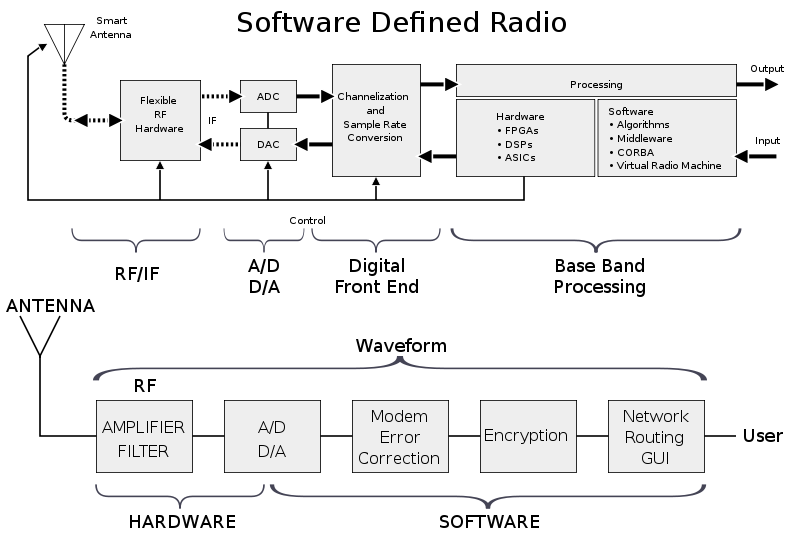
\includegraphics[scale=0.33]{sdrDiagram}
		\caption{Diagramma blocchi funzionamento SDR \cite{sdrDiagram}}\label{fig:1}
	\end{minipage}\hfill
	\begin{minipage}[b]{.4\columnwidth}
		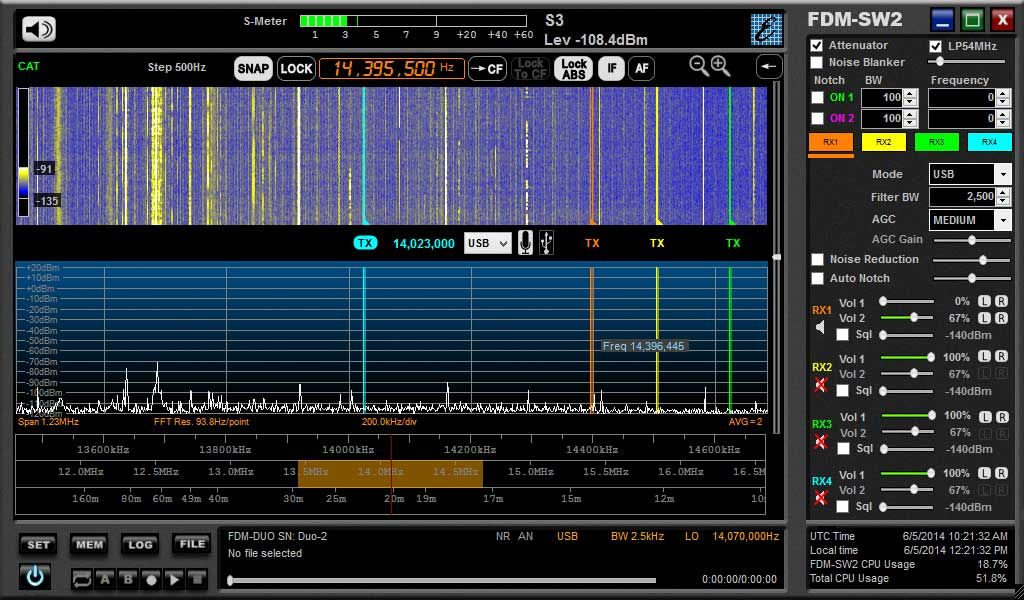
\includegraphics[scale=0.2]{sdrSoftware}
		\caption{Software generico per l analisi dello spettro \cite{sdrSoftware}}\label{fig:1}
	\end{minipage}\hfill
\end{figure}
\newpage
\item \subsection{USRP (Universal Software Radio Peripheral)} URSP è una tipologia di SDR venduta dal marchio Etthus Research pensata per essere accessibile a tutti. Alcune versioni contengono un processore su cui può essere caricato del software per funzionare in autonomia. Sono disponibili anche modelli con una scheda ethernet integrata per il controllo remoto attraverso una rete locale o pubblica. Gli USRP permettono la trasmissione e la ricezione contemporaneamente e dispongono di un ampio range di frequenze che varia in relazione al modello ma è di gran lunga più elevato rispetto agli sdr-rtl. Le schede USRP sono utilizzabili con il driver UHD, disponibile sottoforma di due blocchi: uno per la ricezione ed uno per la trasmissione, pronti per essere integrati nel proprio flusso su Gnuradio.
\subsubsection{Ettus USRP-B210}
Questo modello del costo di 1100 euro in dotazione ai laboratori dell' università permette di variare la frequenza da 70MHz a 6GHz e raggiungere una frequenza di campionamento di 56MHz. Supporta MIMO in full-duplex
\begin{figure}[h]
	\centering
	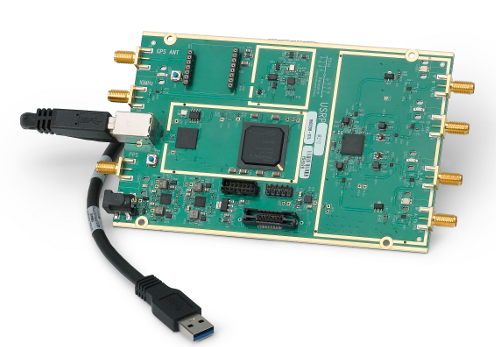
\includegraphics[scale=0.45]{B210}
	\caption{USRP modello B210\cite{b210}}\label{fig:1}
\end{figure}

\item \subsection{RTL-SDR} Questa particolare tipologia di SDR sono i più economici presenti sul mercato, vengono venduti come decoder per lo standard DVB-T della televisione digitale e per DAB e FM della radio. Utilizzando driver alternativi è possibile ricevere un flusso di campionamenti dalla scheda. Questa tipologia di SDR è solo in grado di ricevere il segnale, inoltre presenta limitazioni sia sulla frequenza di ricezione (minore di 2GHz) che sulla frequenza di campionamento (minore di 2MHz per una lettura affidabile, fino a 3Mhz).
\begin{figure}[h]
	\centering
	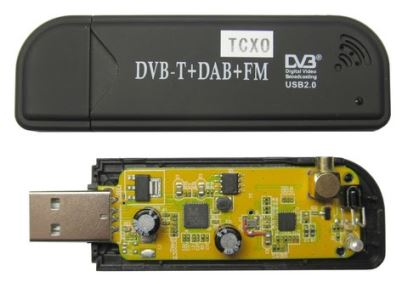
\includegraphics[scale=0.55]{rtlsdr}
	\caption{RTL-SDR venduto come ricevitore DVB-T, DAB e FM\cite{rtlsdr}}\label{fig:1}
\end{figure}

\chapter{Gnuradio}
GNU Radio è una piattaforma gratis e open-source per lo sviluppo di codice finalizzato all'implementazione di software radio. Lo sviluppo può essere eseguito sia utilizzando schede hardware esterne oppure simulando lo scenario virtualmente. Il progetto GnuRadio è nato nel 2001 con l'idea di portare il concetto di free-software anche nel mondo delle Software Defined Radio visto che in precedenza questo settore era dominato solo da software proprietari. Attualmente è molto utilizzato sia in ambito accademico che commerciale e negli ultimi anni anche nel mondo hobbistico. Lo sviluppo in GnuRadio consiste nella disposizione di una serie di blocchi ciascuno dei quali svolge un operazione ben precisa. Il collegamento fra i blocchi è monodirezionale e rappresenta il flusso delle informazioni dalla sorgente al pozzo finale.

 Il programma ufficiale dispone di molti moduli per l' elaborazione delle informazioni e l' interazione esterna, tuttavia è possibile creare un proprio blocco da inserire nel flusso con il linguaggio python oppure C++. Per creare un blocco personalizzato Gnuradio mette a disposizione pyBOMBS il cui compito è quello di preparare l'ambiente per lo sviluppo e l'integrazione del blocco scaricando e configurando le librerie necessarie senza che l'utente debba preoccuparsene.
 Per la creazione di tutti i file necessari per il funzionamento di un blocco viene fornita l'utility gr\_modtool che attraverso riga di comando guida l'utente sulla configurazione dei parametri necessari. Un modulo Gnuradio deve possedere delle caratteristiche standard stabilite per il corretto funzionamento. Ogni blocco deve specificare che tipologia di valori aspetta in ingresso ed in uscita (Int, Float, Complex, ecc.), quanti ingressi e uscite fornirà, la lista dei parametri da richiedere all'utente per l'utilizzo e il rapporto fra il numero di campioni in ingresso e quello in uscita. I blocchi dunque devono avere un rapporto costante fra input e output rappresentato da una costante. Il tool gr\_modtool permette la creazione (se lo sviluppatore lo specifica) di un file python per il testing (Quality assurance). Eseguendo il file di test viene simulato un semplice diagramma come se fosse stato creato nell'ambiente grafico, questo diagramma è personalizzabile e permette di aggiungere tutti i blocchi necessari. Solitamente è sufficiente avere un diagramma composto da tre blocchi: il primo per fornire le informazioni al blocco sotto test, il blocco stesso ed infine un blocco che ritorna i risultati ottenuti permettendo al codice di confrontarli con quelli desiderati.
 Una volta completato lo sviluppo è possibile compilare il blocco per renderlo utilizzabile all' interno dell'ambiente Gnuradio.

\chapter{Crittografia RSA}
L'algoritmo RSA (Rivest–Shamir–Adleman) è un algoritmo per la criptazione ampiamente utilizzato che basa il suo funzionamento sulla difficoltà di fattorizzare un numero generato moltiplicando due numeri primi grandi. La base matematica dell' algoritmo venne pubblicata nel 1976 da due matematici Diffie e Hellman, famosi per aver inventato l'algoritmo Diffie-Hellman, utilizzato ancora oggi per instaurare una crittografia a chiave simmetrica ma senza la trasmissione della chiave. L'algorito RSA venne pubblicato nel 1977 tuttavia era già stato segretamente documentato da un matematico  militare britannico qualche anno prima ma venne mantenuta la notizia segreta fino al 1997.
 
\section{Caratteristiche}
\begin{itemize}
\item \subsection{Codifica asimmetrica con doppia chiave} Le due chiavi sono dette privata e pubblica e vengono generate dallo stesso dispositivo, poi viene pubblicata solo quella pubblica. RSA è un algoritmo a chiave asimmetrica che utilizza quindi due chiavi distinte per la procedura di codifica e decodifica, a differenza degli algoritmi a chiave privata condivisa in RSA. La chiave privata è posseduta solo da uno dei due soggetti della comunicazione rendendone più difficile l'ottenimento da parte di un eventuale attaccante.\cite{brunato}
\item \subsection{Algoritmo unico}
RSA utilizza lo stesso algoritmo per la codifica e la decodifica delle informazioni.\cite{brunato}
\item \subsection{Chiavi intercambiabili}
E' possibile utilizzare le chiavi nell'ordine preferito, ad esempio durante l'invio di un messaggio il trasmettitore lo codificherà con la chiave pubblica del ricevitore mentre per le firme digitali il trasmettitore cripterà un hash del messaggio con la propria chiave privata permettendo al ricevitore di verificare l'identità.\cite{brunato}
\item \subsection{Procedimento creazione chiave monodirezionale} E' computazionalmente semplice generare la chiave pubblica partendo da quella privata mentre il contrario è proibitivo. Non è matematicamente dimostrata l'impossibilità della scoperta di un algoritmo che renda la procedura inversa efficiente.\cite{brunato}
\end{itemize}

\section{Algoritmo}
\begin{itemize}
\item \subsection{Generazione delle chiavi}
Il primo passo consiste nel generare la chiave privata e quella pubblica. Tutta la seguente procedura viene effettuata solo su un dispositivo.
 \begin{itemize}
	\item vengono scelti due numeri primi molto grandi con lunghezza simile e ne viene eseguita il prodotto \( n = p*q \), n sarà il modulo utilizzato nell' algoritmo di codifica/decodifica
	\item viene calcolato \(f(n) = (q-1)*(p-1)\)
	\item viene scelto un numero e tale che \(1<e<f(n)\) e che \(MCD(e,f(n))=1\)
	\item viene calcolato \(d = e^{-1} \, mod \, f(n)\) utilizzando l'algoritmo di euclide
\end{itemize}
La chiave pubblica sarà formata dalla coppia (e,n) mentre quella privata (d,n). \cite{rsa}
\item \subsection{Cifratura} La cifratura verrà eseguita dal mittente utilizzando la chiave pubblica resa nota dal destinatario (e,n) calcolando \(C = M^e \, mod \, n\).
\cite{rsa}
\item \subsection{Decifratura} La decifratura verrà eseguita dal destinatario con la propria chiave privata (d,n) decodificando il messaggio \(M = C^d \, mod \,  n\).
\cite{rsa}
\end{itemize}


\newpage